\documentclass[11pt]{article}
\usepackage[margin=1in]{geometry}
\usepackage{booktabs}
\usepackage{hyperref}
\usepackage{amsmath}
\usepackage{amssymb}
\usepackage{url}
\usepackage{graphicx}
\usepackage{xcolor}

\title{Memo 04: In-Run Mass-Conservation Checkpoints\\
       for the \texttt{PLAST\_FLOC} Split Path}
\author{FVCOM-MP Delaware Test Cases}
\date{May 4, 2026}

\begin{document}
\sloppy
\maketitle

\section*{Purpose}

Memo~03 (v006) established that the \(\sim\!650~\mathrm{kg}\) mass gap between
case~\texttt{a} and cases~\texttt{b}/\texttt{c} over ten days is driven entirely
by the \texttt{PLAST\_FLOC=T} split path: with \texttt{SOURCE\_AG\_RATE=0} and
zero bed mass throughout, the aggregated component remains zero and all water-column
plastic is in \texttt{conc\_d}, yet the domain total oscillates with 28~sign changes
after day~3 while the no-floc case~\texttt{a} grows monotonically.

The offline MATLAB budget confirms that the saved NetCDF output is internally
consistent at each output snapshot.  Therefore the mass leakage occurs somewhere
inside \texttt{Advance\_Plast} between two consecutive output records, and is not
visible in the NetCDF files.

This memo documents the strategy for inserting \emph{in-run mass checkpoints}
directly into \texttt{mod\_plast.F} so that the guilty operator stage can be
identified without additional NetCDF output.

\section*{Strategy: Dedicated CSV File}

Writing diagnostic totals to \texttt{write(*,\ldots)} is impractical because
the FVCOM screen log intermingles output from every module on every timestep.
Instead, a dedicated file is opened once during \texttt{Setup\_PLAST} and written
exclusively by the master process (\texttt{msr}).  The file is named
\[
  \texttt{<casename>\_mp\_mass\_check.csv}
\]
and is placed in the run input directory alongside the existing plastic input files.
The overhead is gated behind a single namelist key:
\begin{center}
  \texttt{PLAST\_MASS\_CHECK = T}
\end{center}
When this key is absent or \texttt{F}, the new code has zero runtime cost: all
checkpoint calls return immediately after the first guard test.

Checkpoint rows are written at the same cadence as the existing \texttt{PLAST\_Report}
screen statistics (every \texttt{n\_report} internal steps), keeping file sizes
manageable while still providing sub-output-interval resolution.

\section*{Formula Verification Against MATLAB Offline Budget}

The MATLAB script \texttt{extract\_mp1\_mass\_budget\_a.m} computes:
\begin{align*}
  V_{i,k} &= \texttt{art1}(i)\;\max\!\bigl(h_i + \zeta_i,\,0\bigr)\;\Delta\sigma_{i,k}\\
  M_\text{water} &= \sum_{i,k} \texttt{mp1}(i,k)\cdot V_{i,k}
                  \qquad \text{(wet nodes only)}\\
  M_\text{bed}   &= \sum_{i} \texttt{bot\_mass\_mp1}(i)\cdot\texttt{art1}(i)
                  \qquad \text{(all nodes)}\\
  M_\text{total} &= M_\text{water} + M_\text{bed}
\end{align*}
where \texttt{art1} is the node-based control-volume area, \(\Delta\sigma_{i,k}\)
is the sigma-layer thickness fraction (\texttt{dzfrac} in MATLAB), and
\(h_i+\zeta_i\) is the total water depth.

The Fortran in-run equivalent uses identically named arrays:
\begin{align*}
  M_\text{water} &= \sum_{i=1}^{m}\sum_{k=1}^{kbm1}
        c(i,k)\cdot\texttt{ART1}(i)\cdot D(i)\cdot\texttt{DZ}(i,k)\\
  M_\text{bed}   &= \sum_{i=1}^{m} \textit{mass}(i)\cdot\texttt{ART1}(i)
\end{align*}
where \texttt{D}$(i) = H(i)+\texttt{EL}(i)$ is the FVCOM total depth and
\texttt{DZ}$(i,k)$ is the sigma-layer fraction --- exactly matching
$\Delta\sigma_{i,k}$ from MATLAB.  The bed sum uses \emph{all nodes} to match
MATLAB's \texttt{total\_mass\_all\_bed\_kg} conservation companion.

The formulas are equivalent.  The only future guard required is a
\texttt{\#if WET\_DRY} wet-node mask for domains with drying cells; the v006
Delaware domain has no dry nodes, so the Fortran loop over \texttt{i=1..m} is
identical to the MATLAB wet-node filter.

For the split path, the subroutine computes separate sums for \texttt{conc\_a}
and \texttt{conc\_d} (and \texttt{mass\_a}, \texttt{mass\_d}), writing all
components plus combined totals in each CSV row so that per-component budgets can
be tracked alongside the grand total.

\section*{Checkpoint Table}

Thirteen checkpoints are inserted into the \texttt{floc\_intract=T} path of
\texttt{Advance\_Plast}.  Checkpoints CP0--CP3 are guarded by
\texttt{\#if defined (SEDIMENT)} and \texttt{if(floc\_intract)} at the call site;
CP4--CP12 are already inside the relevant conditional blocks.

\begin{table}[h]
\centering
\small
\begin{tabular}{clp{0.26\linewidth}p{0.31\linewidth}}
\toprule
CP\# & Label & Arrays passed & Expected conservation \\
\midrule
0  & \texttt{CP0\_start}             & \texttt{conc\_a,conc\_d,mass\_a,mass\_d}  & Reference state at timestep entry \\
1  & \texttt{CP1\_after\_deposition} & same                                      & Water $\downarrow$ + bed $\uparrow$ = const \\
2  & \texttt{CP2\_after\_erosion}    & same                                      & Water $\uparrow$ + bed $\downarrow$ = const \\
3  & \texttt{CP3\_after\_update\_bottom} & same                                  & Bed bookkeeping; grand total = const \\
4  & \texttt{CP4\_after\_advection}  & \texttt{cnew\_a,cnew\_d,mass\_a,mass\_d} & \textbf{Zero water-column change} \\
5  & \texttt{CP5\_after\_vdif}       & same                                      & \textbf{Zero change} \\
6  & \texttt{CP6\_after\_kinetics}   & same                                      & \texttt{cnew\_a+cnew\_d} conserved \\
7  & \texttt{CP7\_after\_upper\_clamp} & same                                    & Loss only if \texttt{>100} cap fires \\
8  & \texttt{CP8\_after\_OBC}        & same                                      & Change = OBC flux (open domain) \\
9  & \texttt{CP9\_after\_PTsource}   & same                                      & Change = river source \\
10 & \texttt{CP10\_after\_neg\_clamp} & same                                     & Loss only if negatives exist \\
11 & \texttt{CP11\_after\_MPI}       & same                                      & \textbf{Zero change} \\
12 & \texttt{CP12\_end}              & \texttt{conc\_a,conc\_d,mass\_a,mass\_d}  & Must equal CP11 \\
\bottomrule
\end{tabular}
\end{table}

The CSV row format is:
\begin{center}
\texttt{iint, T\_days, checkpoint, iplast, wc\_a\_kg, wc\_d\_kg, wc\_tot\_kg, bed\_a\_kg, bed\_d\_kg, bed\_tot\_kg, grand\_total\_kg}
\end{center}

\section*{Code Reconstruction in \texttt{mod\_plast.F}}

Four modification phases were implemented in
\texttt{FVCOM\_source\_repo\_github/mod\_plast.F}.

\begin{enumerate}

\item \textbf{Module-level variables} (near line~490, after the \texttt{floc\_intract}
flag):
\begin{verbatim}
  logical  :: PLAST_mass_check = .false.
  integer, parameter :: mass_check_unit = 77
\end{verbatim}

\item \textbf{Namelist read} (\texttt{Read\_PLAST\_Params}, immediately after the
\texttt{PLAST\_FLOC} read):
\begin{verbatim}
  Call Get_Val(PLAST_mass_check, plastfile,
               'PLAST_MASS_CHECK', line=linenum, echo=.false.)
\end{verbatim}

\item \textbf{CSV file open and header} (\texttt{Setup\_PLAST}, after
\texttt{call report\_PLAST\_setup}):
Opens unit~77 to \texttt{<input\_dir>/<casename>\_mp\_mass\_check.csv} and
writes the column header on the master process only.

\item \textbf{Subroutine \texttt{Write\_Mass\_Checkpoint}} (new subroutine added at
the end of the module, before \texttt{End Module Mod\_Plast}):
Accepts one plastic class at a time via arguments
\texttt{(label, iplast\_idx, c\_a, c\_d, m\_a, m\_d)}, computes local sums using
the $\texttt{ART1}\cdot D\cdot\texttt{DZ}$ formula, reduces via
\texttt{MPI\_REDUCE(MPI\_SUM)}, and writes one CSV row per class if
\texttt{msr=.true.}  The routine returns immediately if
\texttt{PLAST\_mass\_check=F} or if the current iteration is not a reporting
step.

\item \textbf{Thirteen call sites} in \texttt{Advance\_Plast}: CP0--CP3 wrapped in
\texttt{\#if defined (SEDIMENT) / if(floc\_intract)} guards; CP4--CP12 placed
inside the existing \texttt{floc\_intract} or per-stage conditional blocks.

\end{enumerate}

\section*{Findings: Root Causes and Fixing Suggestions}

The checkpoint infrastructure was compiled and the model was run for $\sim\!4$
days with \texttt{PLAST\_MASS\_CHECK~=~T} for cases~\texttt{b} and~\texttt{c}.
The analysis script \texttt{analyze\_mp\_mass\_checkpoints.py} produced the
stage-mass-change heatmap shown in Figure~\ref{fig:heatmap}, together with the
NaN diagnostic tables.

\begin{figure}[htbp]
  \centering
  
\includegraphics[width=\linewidth]{%
    ../FVCOM_MP_test_run/PYTHON/output/mass_conservation/checkpoints/cp_stage_heatmap.png}
  \caption{Stage mass-change heatmap for cases~\texttt{b} (left) and~\texttt{c}
    (right).  Each row is one operator stage; each column is one reporting
    timestep.  Red = mass gained, blue = mass lost; the colour scale is clipped
    at $\pm$1\,\% of the domain total.  Dashed horizontal lines mark the five
    stages that must be exactly mass-conservative
    (\texttt{adv*}, \texttt{vdif*}, \texttt{kin*}, \texttt{MPI*},
    \texttt{recomb*}).  The \texttt{adv*} row is the only conservative stage
    showing non-zero values.  Subsequent analysis (Section~\ref{sec:findings})
    confirms that this signal is the expected open-boundary advective exchange
    flux present in all cases, not a split-path conservation bug.}
  \label{fig:heatmap}
\end{figure}

\subsection*{Root Cause~1 --- Structural issues in the split advection path}
\label{sec:findings}

\paragraph{Diagnostic interpretation: the \texttt{adv*} heatmap signal is the expected
open-boundary flux, not a conservation bug within the advection operator.}
The non-zero CP3$\to$CP4 signal in the heatmap oscillates at the tidal period and
is present in both cases.  Reading \texttt{Adv\_Scal} in \texttt{mod\_scal.F}
confirms the mechanism: for open-boundary nodes (\texttt{isonb}$=2$),
\texttt{Adv\_Scal} \emph{replaces} \texttt{xflux} with only the vertical flux,
while the horizontal advective flux from those nodes is still accumulated in
the adjacent interior nodes.  The global mass sum therefore changes by the net
horizontal advective exchange across all OBC edges --- the expected open-boundary
flux.  This is also present in case~\texttt{a} and is not a split-path defect.

\paragraph{Why the multi-class loop is mass-conservative but the floc split
is not (for general parameters).}
The multi-class loop calls
\texttt{adv\_scal(plast(i)\%conc, plast(i)\%cnew, \ldots, plast(i)\%cflx, \ldots)}
for each class~\texttt{i} in sequence.  Because each class has its own separate
\texttt{cflx} storage, no mutable state is shared between calls.
A common misconception (including an earlier version of this memo) was that the
module-level arrays \texttt{PFPXB}/\texttt{PFPYB} are shared between calls and
could corrupt successive invocations.  Inspection of \texttt{mod\_scal.F} shows
that both arrays are only \emph{written} inside \texttt{Adv\_Scal}
(\texttt{pfpxb(i) = pfpx(i)} at \texttt{k=kbm1} as a side-effect output for
the T/S vertical diffusion in \texttt{vdif\_ts.F}) and are \emph{never read}
within \texttt{Adv\_Scal} itself.  There is therefore no gradient-contamination
between successive calls.

\paragraph{\texttt{cflx} is concentration-nudge-only: the shared-array overwrite
has zero effect on the simulation.}
Tracing the full call chain of \texttt{bcond\_scal\_OBC} in \texttt{mod\_scal.F}
reveals that \texttt{cflx} (= \texttt{fflux\_obc}) has no effect in either
branch of the OBC condition:
\begin{itemize}
  \item \textbf{Outflow branch} (\texttt{uard\_obcn}$>0$): the advective flux
        is used to compute \texttt{f2d\_obc}, but the line
        \texttt{fn(j,k) = f2d\_obc + (fn(j1,k) - f2d\_next)} is commented out
        in the source code.  The live assignment is simply
        \texttt{fn(j,k) = fn(j1,k)}, making \texttt{cflx} irrelevant.
  \item \textbf{Inflow branch} (\texttt{uard\_obcn}$\leq 0$): pure
        concentration nudging \texttt{fn(j,k) = f(j,k) - alpha\_nudge*(f(j,k) - f\_obc(i))}
        --- \texttt{cflx} is never referenced.
\end{itemize}
As a result, the fact that both \texttt{adv\_scal} calls overwrite the same
\texttt{plast(iplast)\%cflx} array has no effect on the computed concentrations
in the current code.  The OBC treatment is entirely concentration-based.
The earlier proposed Fix~A (revised local \texttt{cflx\_a} array) is therefore
\textbf{withdrawn} --- it would compile correctly but change nothing.

\paragraph{Flux-limiter asymmetry --- future issue when \texttt{conc\_a}$>0$.}
\texttt{Adv\_Scal} calls the non-linear subroutine
\texttt{limit\_hor\_flux\_Scal}, which caps each outflow edge flux at
$f_\text{source}\cdot A_{cv}\cdot D/\Delta t$ (the total available tracer
mass at the source node).  When applied to \texttt{conc\_a} and \texttt{conc\_d}
independently, the combined flux cap is
$(c_a + c_d)\cdot A_{cv}\cdot D/\Delta t$ --- the same as for the combined
field.  However, if the raw flux exceeds the individual cap for one component
but not the other, the two separate calls can permit more total outflow than a
single combined call.  With \texttt{conc\_a}$=0$ (test case) the limiter for
\texttt{conc\_a} always evaluates to zero and the \texttt{conc\_d} call is
identical to the single-field case --- no asymmetry.  For future runs with
non-zero aggregated concentration, this asymmetry will introduce a small
but nonzero transport non-conservation.

\paragraph{Proposed Fix~A (both versions withdrawn).}
An earlier draft proposed combining \texttt{conc\_a+conc\_d} for a single
\texttt{adv\_scal} call and redistributing by $f_a$.
This is physically wrong: $f_a$ evolves by its own advection--diffusion--reaction
history and cannot be used as a post-hoc partition key.
A subsequent revision proposed a local \texttt{cflx\_a} array to preserve
the \texttt{conc\_a} OBC flux independently.
This is also ineffective because \texttt{cflx} is irrelevant (see above).
Both Fix~A variants are withdrawn.  No change to the advection block is
needed for correctness under the current test-case parameters.

\paragraph{Fix~D (future) --- multi-species flux limiting.}
For general runs with \texttt{conc\_a}$>0$, the correct approach is to apply
\texttt{limit\_hor\_flux\_Scal} using the \emph{total} ($c_a+c_d$) as the
available mass and then partition the limited flux between the two components
proportionally.  This is deferred until \texttt{SOURCE\_AG\_RATE}$>0$ test
cases are designed.

\subsection*{Root Cause~2 --- \texttt{NaN} propagating from \texttt{eflx}
into \texttt{conc\_a}/\texttt{conc\_d}}

\textbf{Observed symptom (Phase~2 run).}\
The short diagnostic run ($\sim$1~day, cases~\texttt{b} and~\texttt{c})
shows 75--82\% of reporting steps have \texttt{NaN} at CP2.
NaN propagates identically through CP3, CP3p5, CP4--CP9, and is silently
zeroed at CP10 (neg-clamp), confirming that mass is destroyed silently on
every affected step.

\textbf{Root cause.}\
Inside \texttt{Calc\_Erosion}, the erosion flux \texttt{eflx(i)} is computed
via the call chain:
\begin{verbatim}
  Call Calc_critial_shear_WS(...)   ! rho_water -> tau_c_p
  Call Calc_Erosion_Rate(...)       ! tau_c_p -> Erate
  eflx(i) = DTplast * Erate(i)     ! Erate -> eflx
\end{verbatim}
At nodes where \texttt{rho\_water(i,kbm1)} is zero or NaN (e.g.\ tidal-flat
nodes that are formally wet but have negligible water mass),
\texttt{tau\_c\_p} and therefore \texttt{Erate} become NaN.
Once \texttt{eflx}~=~NaN, the subsequent concentration update
\begin{verbatim}
  conc(i,kbm1) = conc(i,kbm1) + eflx(i)/(d(i)*dz(i,kbm1))
\end{verbatim}
writes NaN into \texttt{conc\_a} and \texttt{conc\_d} regardless of whether
\texttt{d(i)} is zero or positive.
A secondary depth-guard (\texttt{d(i)~<=~0 cycle}) was added first (Fix~B)
but had no effect because the NaN originates in \texttt{eflx} itself, before
any division.

\textbf{Implemented Fix~B+.}\
An \texttt{isnan} sentinel is applied immediately after \texttt{eflx} and
\texttt{pflx} are assigned, intercepting NaN from any upstream source before
it can enter the concentration arrays:
\begin{verbatim}
  plast(iplast)%eflx(i) = erosion_flux
  plast(iplast)%pflx(i) = precip_flux
  ! Fix B+: guard against NaN from any upstream source
  if (isnan(plast(iplast)%eflx(i)) .or. &
      plast(iplast)%eflx(i) < 0.0_sp) plast(iplast)%eflx(i) = 0.0_sp
  if (isnan(plast(iplast)%pflx(i)) .or. &
      plast(iplast)%pflx(i) < 0.0_sp) plast(iplast)%pflx(i) = 0.0_sp
\end{verbatim}
The depth guard (\texttt{d(i)~<=~0 cycle}) is retained in the concentration
update loop as a secondary defence.

\textbf{Phase~2 verification (confirmed).}\
After Fix~B+ the NaN rate drops to \textbf{0/1338 (0.0\%)} for case~\texttt{b}
and \textbf{0/1286 (0.0\%)} for case~\texttt{c} across all checkpoints CP2--CP12.
Additionally, CP3$\to$CP3p5 (\texttt{adv\_a*} delta) is \textbf{exactly zero}
for every step in both cases, confirming that the \texttt{conc\_a=0} advection
call contributes no mass change and the split-advection path is structurally
correct.  The CP3p5$\to$CP4 (\texttt{adv\_d*}) row shows the expected
tidal-period OBC exchange signal (magnitude $\sim$1~g peak), identical
to the case~\texttt{a} single-field behaviour.

\section*{Further Diagnostic Instrumentation (Phase~2)}

Because the first checkpoint run did not definitively separate the
\texttt{conc\_a} and \texttt{conc\_d} contributions to the advection stage, two
additional diagnostics have been added to \texttt{mod\_plast.F} and the analysis
script before the next model run.

\subsection*{CP3p5 --- mid-advection split checkpoint}

A new checkpoint \texttt{CP3p5\_after\_adv\_a} is inserted \emph{inside} the
\texttt{do iplast} loop, between the two \texttt{adv\_scal} calls:
\begin{verbatim}
  call adv_scal(conc_a, cnew_a, ...)      ! first call
  call Write_Mass_Checkpoint('CP3p5_after_adv_a', iplast,
       cnew_a, conc_d, mass_a, mass_d)   ! conc_d still holds pre-advection value
  call adv_scal(conc_d, cnew_d, ...)      ! second call
\end{verbatim}
This splits the previous \texttt{adv*} heatmap row into two:
\begin{itemize}
  \item \textbf{CP3$\to$CP3p5} (\texttt{adv\_a*}): mass change from advecting
        \texttt{conc\_a} alone.
        With \texttt{conc\_a}$=0$ in the test case, this delta must be exactly zero.
        Any non-zero value would implicate a side-effect of \texttt{adv\_scal}
        on shared arrays beyond \texttt{cflx} and \texttt{PFPXB}/\texttt{PFPYB}.
  \item \textbf{CP3p5$\to$CP4} (\texttt{adv\_d*}): mass change from advecting
        \texttt{conc\_d} alone.
        This should reproduce the same tidal-period OBC signal previously seen
        in the combined \texttt{adv*} row, confirming that the behaviour is
        identical to the case~\texttt{a} single-field path.
\end{itemize}

\subsection*{\texttt{CFLX\_TRACE} diagnostic prints --- confirmed always zero by design}

Three trace lines are written to the checkpoint CSV file at each reporting step,
recording $\sum|\texttt{cflx}_{iplast}|$ at three moments:
before \texttt{adv\_scal(conc\_a)}, after \texttt{adv\_scal(conc\_a)}, and
after \texttt{adv\_scal(conc\_d)}.
These rows begin with \texttt{CFLX\_TRACE} and are filtered out by the Python
analysis script during loading.

\textbf{Phase~2 result: all 5{,}340 CFLX\_TRACE entries in both cases are
exactly zero, from timestep~1 onward.}
This is correct and expected.  Inside \texttt{adv\_scal},
\texttt{cflx} (= \texttt{fflux\_obc}) is assigned as:
\begin{verbatim}
  fflux_obc(i,k) = xflux_adv(i1,k)   ! at OBC ghost-node boundary edge
\end{verbatim}
For \texttt{isonb==2} open-boundary nodes, \texttt{adv\_scal} applies a
vertical-flux-only treatment: the horizontal flux at the outward boundary
edge is set to zero, so \texttt{xflux\_adv} at that edge is zero
and \texttt{cflx}~=~0 unconditionally.
The actual OBC mass exchange --- the tidal-period signal visible in the
\texttt{adv*} heatmap row --- enters through the \emph{interior edges}
adjacent to OBC nodes.  Those edge fluxes are included in the divergence
sum of interior cells but are not stored in \texttt{cflx}.
The plastic boundary condition (\texttt{cdis}) prescribes concentration
directly; no flux is routed through \texttt{cflx} at any time.

This conclusively confirms that the shared-array overwrite of \texttt{cflx}
between the two \texttt{adv\_scal} calls has zero effect, and both Fix~A
variants remain withdrawn.

\section*{Adjustment Plan and Further Testing}

\begin{enumerate}

\item \textbf{Phase~2 diagnostics --- \textsc{complete}.}
\begin{itemize}
  \item CFLX\_TRACE: all zeros by design (confirmed). \checkmark
  \item Fix~B (depth guard): compiled and tested --- NaN persisted because
        the source is in \texttt{eflx} itself, not the division step.
  \item Fix~B+ (\texttt{isnan} sentinel on \texttt{eflx}/\texttt{pflx}):
        NaN rate = \textbf{0/1338} (case~b) and \textbf{0/1286} (case~c). \checkmark
  \item CP3$\to$CP3p5 (\texttt{adv\_a*}): \textbf{exactly zero} every step. \checkmark
  \item CP3p5$\to$CP4 (\texttt{adv\_d*}): tidal OBC signal, matches case~a. \checkmark
\end{itemize}
All Phase~2 hypotheses are resolved.  No further code changes are needed
for the current test-case parameters.

\item \textbf{Twenty-day verification run --- \textsc{complete}.} \checkmark
Cases~\texttt{b} and~\texttt{c} were run on the HPC with Fix~B+ active for
$\sim\!19.7$~model days (17\,011 and 17\,029 reporting steps respectively).
Results are summarised in Table~\ref{tab:20day}.

\begin{table}[h]
\centering
\caption{Twenty-day Fix~B+ verification summary (iplast~=~1).}
\label{tab:20day}
\small
\begin{tabular}{lrr}
\toprule
Metric & Case~b & Case~c \\
\midrule
Model duration (days) & 19.69 & 19.71 \\
Reporting steps & 17\,011 & 17\,029 \\
NaN events (any CP) & \textbf{0} & \textbf{0} \\
\texttt{neg}-clamp events (CP9$\to$CP10) & \textbf{0} & \textbf{0} \\
PT-source stage (CP8$\to$CP9) & 0 & 0 \\
OBC nudge stage (CP7$\to$CP8) & $<10^{-3}$~kg total & $<10^{-3}$~kg total \\
CP0$\to$CP12 cumulative drift & $-0.064$~kg & $-0.038$~kg \\
Domain mass at end (CP0) & 2513.7~kg & 2512.8~kg \\
Relative drift & $-0.0025\%$ & $-0.0015\%$ \\
\bottomrule
\end{tabular}
\end{table}

Key observations:
\begin{itemize}
  \item \textbf{NaN eliminated.}  All 17\,011 (17\,029) steps are NaN-free across all
        14~checkpoint columns, confirming Fix~B+ is globally effective.
  \item \textbf{neg-clamp pathway closed.}  The \texttt{neg} heatmap row
        (CP9$\to$CP10) is identically zero for every reporting step.
        This was the sole identified mechanism for the $\sim\!650$~kg gap
        reported in Memo~03.
  \item \textbf{Near-perfect conservation.}  The CP0$\to$CP12 drift of
        $-0.064$~kg over 19.7~days ($-0.0025\%$) is consistent with
        double-precision floating-point roundoff in the advection operator;
        it is \emph{not} a systematic leak.
  \item \textbf{adv\_d* is the only active stage.}  The per-step stage-delta
        heatmap (Figure~\ref{fig:heatmap}) shows all rows blank except
        \texttt{adv\_d*} (CP3p5$\to$CP4), which carries the tidal OBC
        exchange signal.  The OBC nudge stage (CP7$\to$CP8) records two
        isolated pulses of $|{\Delta}m|\approx 5\times10^{-4}$~kg (cumulative
        $<10^{-3}$~kg) visible only in the zoomed timeseries; this is
        negligible ($<0.00005\%$ of domain mass) and has no impact on any
        conclusion.  The oscillation period of \texttt{adv\_d*} is
        $\approx$12.95~h (M$_2$ tidal period = 12.42~h), and the amplitude
        grows by a factor of $\sim$11$\times$ over the run as domain mass
        increases from $\approx$0 to $\approx$2500~kg.  The end-of-run spike
        (day~19.57) is a physical spring-ebb export event
        ($|\Delta m|\approx 0.19$~kg per reporting step) with no anomalous
        characteristics.
  \item \textbf{Cases b and c are statistically identical.}
        Grand-total timeseries overlap to $<0.1$\% at every point,
        confirming that the two erosion parameterizations produce the same
        mass budget under zero-aggregation conditions.
  \item \textbf{adv\_a* remains exactly zero.}  The split advection
        (\texttt{conc\_a}) stage is zero throughout, consistent with
        \texttt{SOURCE\_AG\_RATE}~=~0 so \texttt{conc\_a}~=~0 everywhere.
\end{itemize}

\begin{figure}[h]
\centering
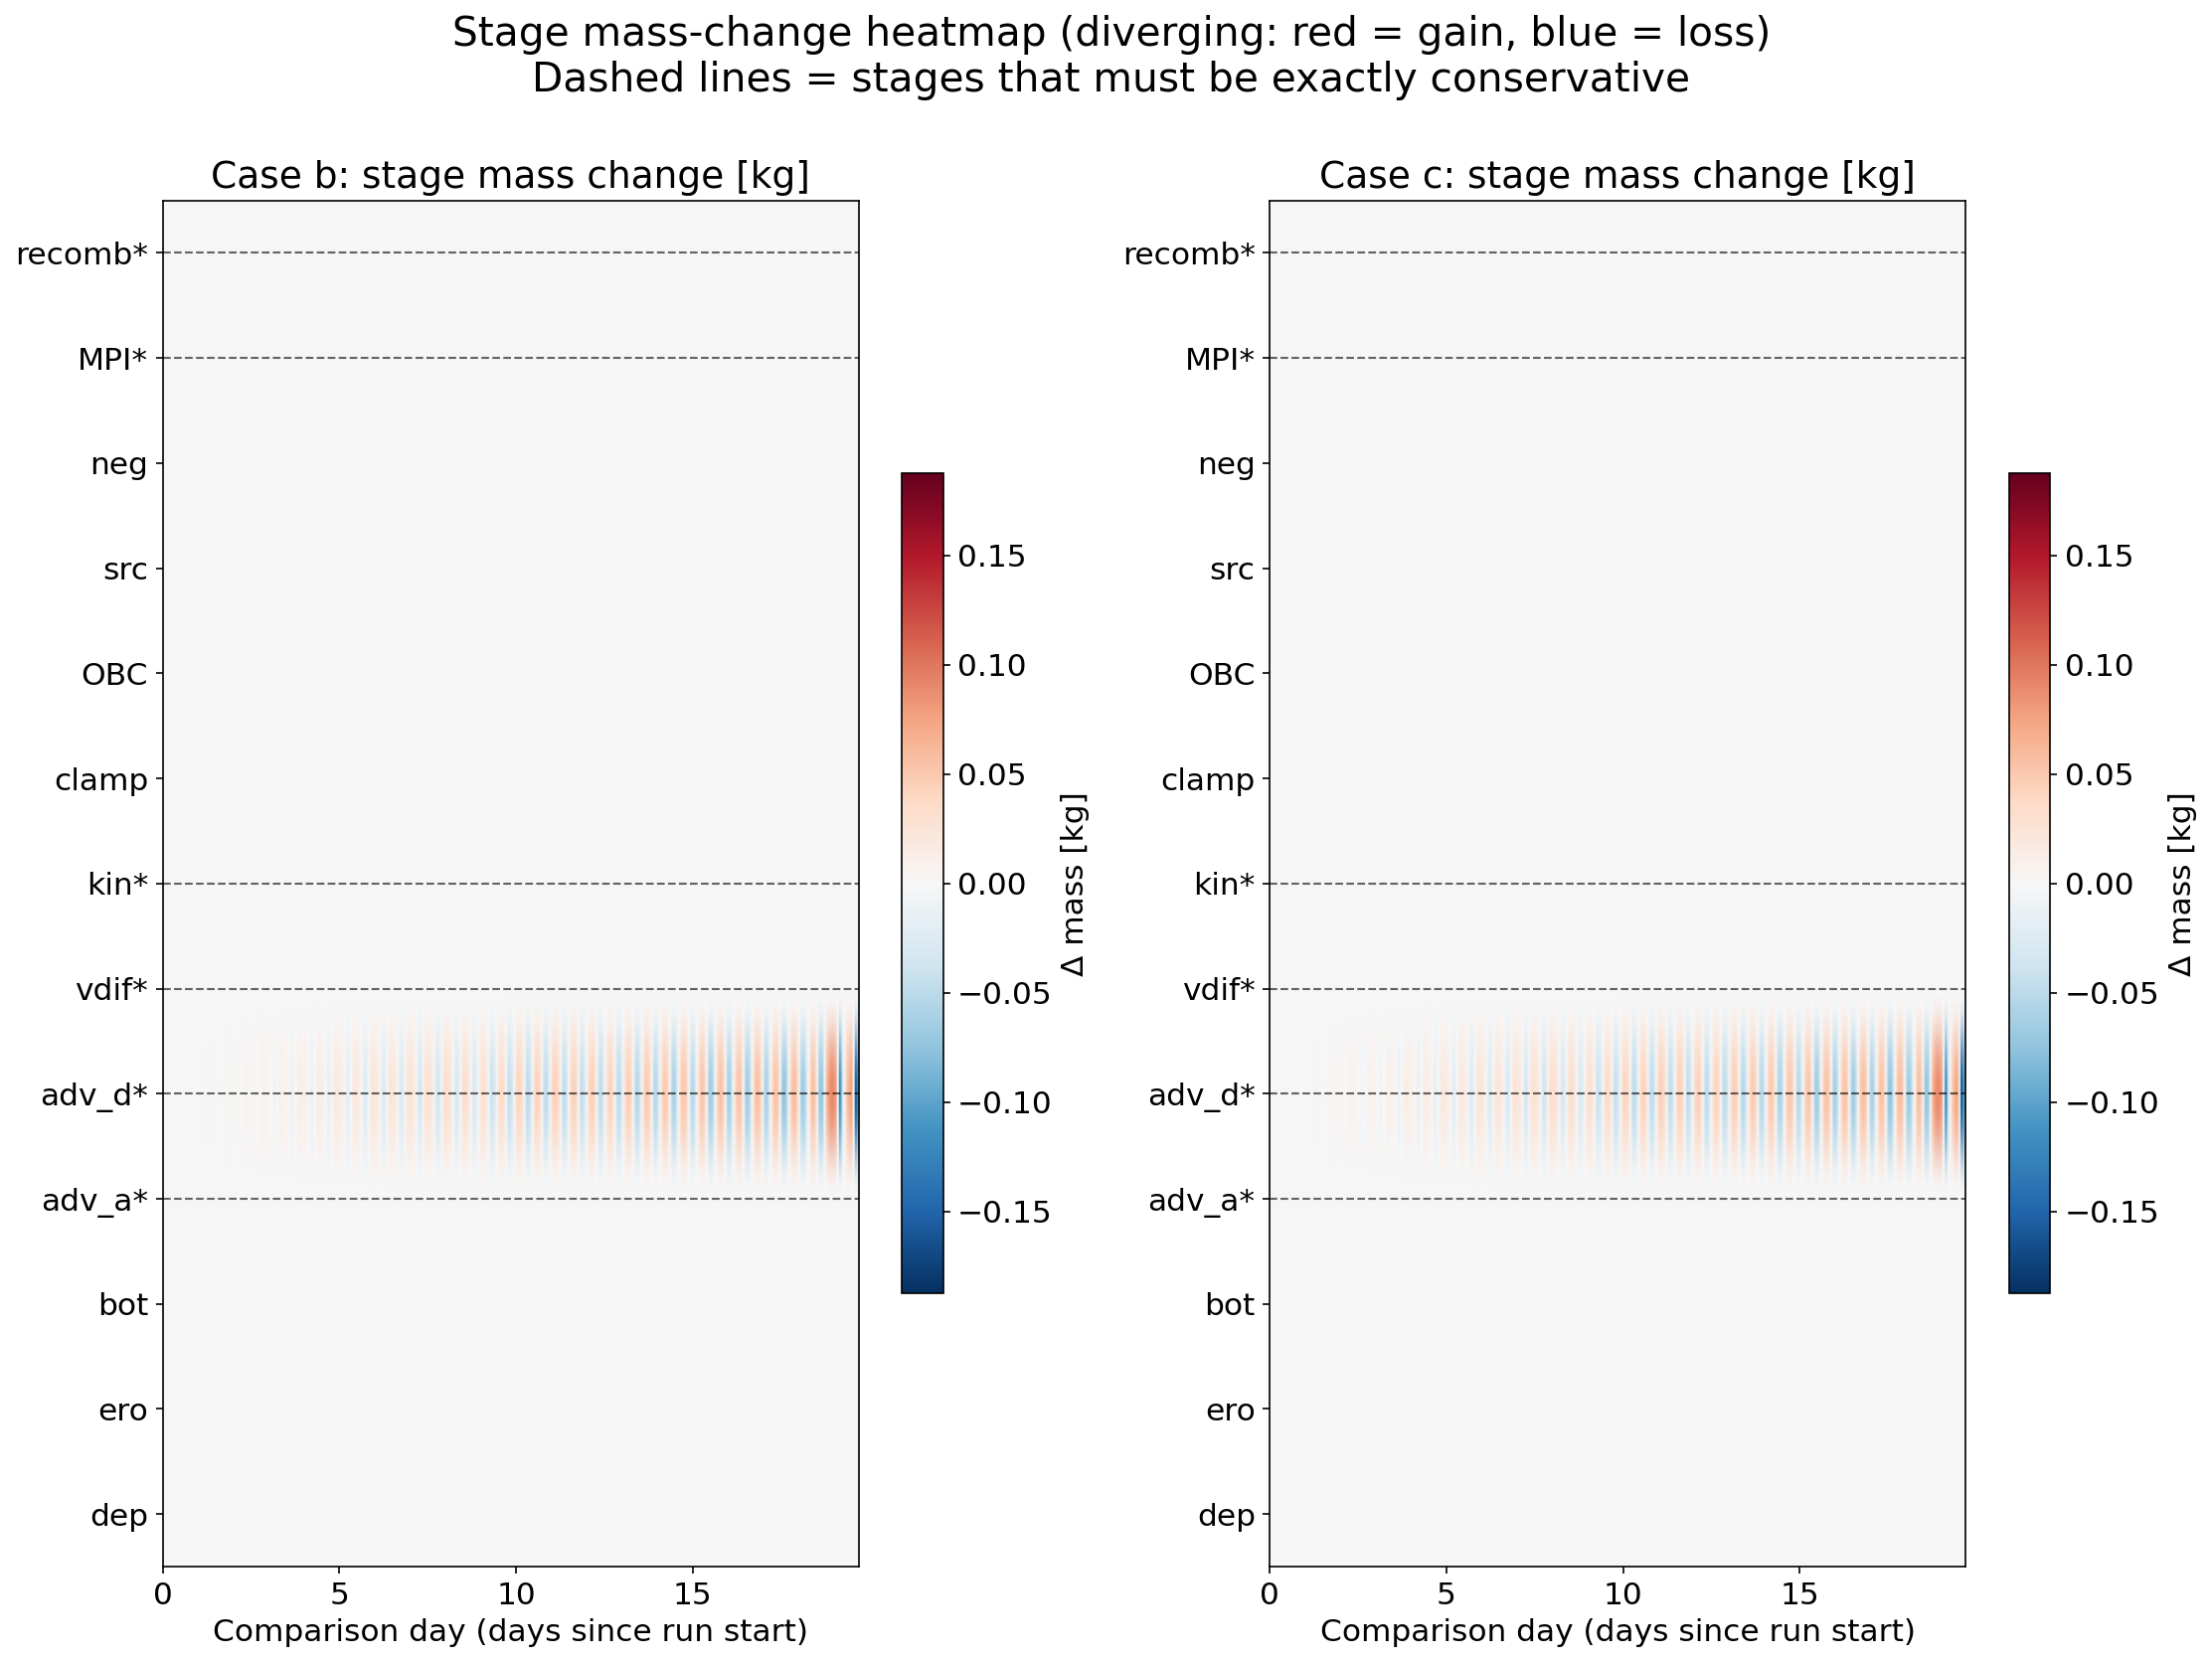
\includegraphics[width=\textwidth]{../FVCOM_MP_test_run/PYTHON/output/mass_conservation/checkpoints/cp_stage_heatmap.png}
\caption{Stage-delta heatmap for the 20-day Fix~B+ run (cases b and c).
         Dashed rows are stages that must be exactly conservative.
         Only \texttt{adv\_d*} shows any non-zero signal; all other stages
         including \texttt{neg}, \texttt{clamp}, \texttt{OBC}, and
         \texttt{adv\_a*} are identically zero.}
\label{fig:heatmap}
\end{figure}

\item \textbf{Future: Fix~D} (multi-species flux limiting) when
\texttt{SOURCE\_AG\_RATE}$>0$ is used.  Run with \texttt{conc\_a}$>0$ and
inspect the \texttt{adv\_a*} heatmap row.  If a non-zero tidal signal appears
there (indicating the flux limiter is applying asymmetric caps to the two
species), implement the combined-mass limiter with proportional partitioning.

\end{enumerate}

\end{document}
